\documentclass{article}
\usepackage[utf8]{inputenc}
\usepackage[a4paper, margin=2.5cm]{geometry}
\usepackage{graphicx}
\usepackage[french]{babel}

\usepackage[default,scale=0.95]{opensans}
\usepackage[T1]{fontenc}
\usepackage{amssymb} %math
\usepackage{amsmath}
\usepackage{amsthm}
\usepackage{systeme}
\usepackage{bbm}
\usepackage{hyperref}
\hypersetup{
    colorlinks=true,
    linkcolor=blue,
    filecolor=magenta,      
    urlcolor=cyan,
    pdftitle={Overleaf Example},
    % pdfpagemode=FullScreen,
    }
\urlstyle{same} %\href{url}{Text}

\theoremstyle{plain}% default
\newtheorem{thm}{Théorème}[section]
\newtheorem{lem}[thm]{Lemme}
\newtheorem{prop}[thm]{Proposition}
\newtheorem*{cor}{Corollaire}
%\newtheorem*{KL}{Klein’s Lemma}

\theoremstyle{definition}
\newtheorem{defn}{Définition}[section]
\newtheorem{exmp}{Exemple}[section]
% \newtheorem{xca}[exmp]{Exercise}

\theoremstyle{remark}
\newtheorem*{rem}{Remarque}
\newtheorem*{note}{Note}
%\newtheorem{case}{Case}



\title{Liste des Tests du cours}
\author{Charles Vin}
\date{2022}

\begin{document}
\maketitle
\tableofcontents

\section{Template}
\subsection*{Donnée}
\subsection*{Conditions}
\subsection*{Hypothèse}
\subsection*{Statistique de test}
\subsection*{Zone de Rejet}
\subsection*{Méthode}

\section{Test d'ajustement de Kolmogorov-Smirnov}


\subsection*{Conditions}
\begin{enumerate}
    \item Les $ X_i $ semblent provenir d'une loi à fonction de répartition continue. $ \Rightarrow  $ on n'a pas plusieurs fois la même valeur (sauf si celle-ci on était arrondi).
    \item Fonctionne $ \forall n $ : même si $ n $ est petit, ce test est pertinent
    \item Si $ n \geq 100 $, on fait un test asymptotique.
\end{enumerate}

\subsection*{Hypothèse}
\begin{itemize}
    \item $ H_0 = $ les $ X_i $ ont pour fdr. $ F_X $ 
    \item $ H_1 = $ les $ X_i $ n'ont pas pour fdr. $ F_X $ 
\end{itemize}

\subsection*{Statistique de test} 
\begin{align*}
    h(F_n, F) &= \sup _{t \in \mathbb{R}} \left| F_n(t) - F(t) \right| \\
        &= \max _{1 \leq i \leq n} ( \max ( \left| \frac{i}{n} - F(X_{(i)}) \right| , \left| \frac{i-1}{n}- F(X_{(i)}) \right|  ))
\end{align*}    

\subsection*{Zone de Rejet}
\subsubsection*{Si n est petit}
La loi de $ h(F_n, F) $ est tabulé alors :
\[
    \mathcal{R} = \{h(F_n, F_X) \geq h_{1-\alpha }\}
.\]
avec $ F_n $ fonction de réparation empirique, $ h_{1 -\alpha } $ le quantile à aller chercher dans la table 

\subsubsection*{Si n est grand $ n \geq 30 $ }
Attention pas souvenir de l'avoir fait en TD. \\
On a pas la table de $ h(F_n, F) $ mais on sait que 
\[
    \sqrt[]{n}h_n \to ^{\mathcal{L}}_{n \to \infty } W_{\infty }
.\]
Donc on pose la zone de rejet 
\[
    \mathcal{R} = \{h(F_n, F_X) \geq \frac{k_\alpha }{\sqrt[]{n}} \}
.\]
avec $ F_n $ fonction de réparation empirique, $ k_{\alpha } $ le quantile de $ W_\infty  $ à aller chercher dans sa table 

\subsection*{Méthode}
Pour trouver la valeur de $ h(F_n, F_X) $ : Faire le grand tableau puis trouver le max. Exemple : 
\begin{table}[!h]
    \centering
    \begin{tabular}{|l|l|l|l|l|l|}
    \hline
        i & 1 & 2 & 3 & 4 & 5 \\ \hline
        $X_{(i)}$ & 0.3 & 0.7 & 0.9 & 1.2 & 1.4 \\ \hline
        $X_{(i)} - 2$ & -1.70 & -1.30 & -1.10 & -0.80 & -0.60 \\ \hline
        $F_0(X_{(i)})$ & 0.04 & 0.10 & 0.14 & 0.21 & 0.27 \\ \hline
        $\frac{i}{n}$ & 0.05 & 0.1 & 0.15 & 0.2 & 0.25 \\ \hline
        $|\frac{i}{n} - F_0(X_{(i)})|$ & 0.01 & 0.00 & 0.01 & 0.01 & 0.02 \\ \hline
        $|\frac{i-1}{n} - F_0(X_{(i)})|$ & 0.04 & 0.05 & 0.04 & 0.06 & 0.07 \\ \hline
    \end{tabular}
    \caption{Ici le max c'est $0.07$ à la dernière case}
\end{table}



\section{Le test du $ \mathcal{X}^2 $ d'ajustement}
\subsection*{Conditions}
\begin{enumerate}
    \item Les $ X_i $ sont à valeur dans un ensemble fini (loi discrète). Si a valeur dans $ \mathbb{N} $, on fusionne les classes à partir d'un certain rang choisis 
    \item Test asymptotique : $ \forall k \in \{1, \dots, d\}, np_k^{ref}(1-p_k^{ref}) \geq 5 \Leftrightarrow n \geq 20$ 
\end{enumerate}
Si on ne remplis pas les conditions, on peut fusionner les classes 

\subsection*{Hypothèse}
\begin{align*}
    H_0 &= p = p^{ref} \text{ i.e. } \forall k \in \{1,\dots,d\}, p_k = p_k^{ref} \\
    H_1 &= p \neq p^{ref} \text{ i.e. } \exists k \in \{1, \dots, d\}: p_k \neq p_k^{ref}
\end{align*}
Avec $ p^{ref} $ un vecteur fixé à tester (par exemple pour un lancé de dé $ (\frac{1}{6}, \dots, \frac{1}{6}) $ )

\subsection*{Statistique de test}
\begin{align*}
    D(\bar{p_n}, p^{ref}) &= n \sum_{k=1}^{d}\frac{(\bar{p_{k,n}} - p_k^{ref})^2}{p_k^{ref}} \to ^{\mathcal{L}}_{n \to \infty } \mathcal{X}^2(d-1) \\
        &= \sum_{k=1}^{d} \frac{(N_{k,n} - np_k^{ref})^2}{n p_k^{ref}}
\end{align*}
avec \begin{itemize}
    \item $ N_{k,n} = \sum_{i=1}^{n}\mathbbm{1}_{X_i x_k} $ (ce qu'il y a dans le tableau de la consigne)
    \item $ \bar{p_{k,n}} = \frac{N_{k,n}}{n} $ les proportions observés
\end{itemize}

\subsection*{Zone de Rejet}
\[
    \mathcal{R} = \{D(\bar{p_n}, p^{ref}) \geq h_\alpha\}
.\]
avec $ h_\alpha  $ le quantile d'ordre $ 1-\alpha  $ de la loi $ \mathcal{X}^2(d-1) $

\subsection*{Méthode}
\begin{enumerate}
    \item Etape 0 : On vérifie les conditions 
    \[
        \forall k \in \{1, \dots, d\}, n*p_k \geq 5
    .\]
    C'est la condition de Cochran (1954), il avait testé cas possible en observant l'approximation faites.
    \item Etape 1 : On calcule les effectifs et proportions observées : $ N_{k,n} $ et $ \hat{p}_{k,n} $  
    \item Etape 2 : Calcul de la statistique de test 
    \[
        D = n \sum_{d}^{k=1} \frac{(\hat{p}_{k,n} - p_k)^2}{p_k}
    .\]
    \item Etape 3 : Détermination de la zone de rejet au niveau $ \alpha  $. On lit $ h_\alpha  $ le quantile d'ordre $ 1-\alpha  $ de la loi $ \mathcal{X}^2(d_1) $ 
    \item Etape 4 : Décisions \begin{itemize}
        \item si $ D > h_\alpha  $, on rejette $ H_0 $ (au niveau $ \alpha  $ ). 
        \item Si $ D \leq h_\alpha  $ on conserve $ H_0 $ 
    \end{itemize}
\end{enumerate}

\subsubsection*{Bilan de la méthode}
Aspects positifs : 
\begin{itemize}
    \item \textbf{Fonctionne pour toutes les lois}
    \item Facile à faire
\end{itemize}

Aspects négatifs : 
\begin{itemize}
    \item Problème de consistance. Regrouper les variables par intervalle ruiner l'erreur de seconde espèce.
    \item Asymptotique
    \item Dépendant du choix des intervalles. Ce qui n'est pas canonique.
\end{itemize}

\subsection{Le $ \mathcal{X}^2 $ d'ajustement à une famille paramétrique de loi}
Pratiquement comme avant, pas encore fait en TD, mais copier collé du cours quand même 
\begin{enumerate}
    \item Etape 1 : Soit $ \hat{\theta }_n $ l'estimateur du maximum de vraisemblance de $ \theta  $ (pour $ P_\theta  $ ). On estime \textbf{tous} les paramètres de la loi $ (p_1^{\hat{\theta }_n}, \dots, p_d^{\hat{\theta }_n}) $ 
    \item Etape 2 : On vas tester l'ajustement de $ X_1, \dots, X_n $ à $ P_{\hat{\theta }_n} $ On calcule les fréquences observées $ \hat{p}_{k,n} $.
    \item Etape 3 : Vérification des conditions $ np_k^{\hat{\theta }_n} $ et possible regroupement en classes 
    \item Etape 4 : Calcul de la stat de test $ D $ 
    \item Etape 5 : Zone de rejet : lecture de $ H_\alpha  $ le quantile d'ordre $ 1-\alpha  $ d'une $ \mathcal{X}^2(d-1-M) $ avec $ M $ nombre de paramètre. 
    \item Etape 6 : Décision 
        \begin{itemize}
            \item $ D > h_\alpha  $ on rejette $ H_0 $ 
            \item $ D \leq h_\alpha  $ on conserve $ H_0 $ 
        \end{itemize}
\end{enumerate}


\section{Le test d'homogénéité de Kolmogorov-Smirnov}
\subsection*{Conditions}
\begin{itemize}
    \item Deux échantillons indépendants de variable iid.
    \item De fdr. continue $ F_X, F_Y $ 
\end{itemize}

\subsection*{Hypothèse}
\begin{itemize}
    \item $ H_0 $ : les $ X_i $ et $ Y_i $ ont la même loi, c'est à dire $ F_{X_1} = F_{V_1} $ où $ F_{X_1}, F_{Y_1} $ sont continues.
    \item $ H_1 $ les lois sont différentes
\end{itemize}

\subsection*{Statistique de test}
\[
    \sup _{s \in \mathbb{R}} \left| \frac{1}{n}\sum_{i=1}^{n} \mathbbm{1}_{X_i \leq t} - \frac{1}{n}\sum_{j=1}^{n} \mathbbm{1}_{Y_j \leq t} \right| 
.\]
\subsection*{Zone de Rejet}
\begin{itemize}
    \item Ce test est de taille $ \alpha  $, si on utilise la table de $ h_{n,m} = \sup _{s \in \mathbb{R}} \left| \frac{1}{n}\sum_{i=1}^{n} \mathbbm{1}_{U_i \leq s} - \frac{1}{n}\sum_{j=1}^{n} \mathbbm{1}_{V_j \leq s} \right| $.
    \item Si $ n $ et $ m $ sont trop grands, on utilise le résultat suivant : \\
        Sous $ H_0 $ 
        \[
            h_{n_1, n_2} = \sqrt[]{\frac{nm}{n+m}}h(F_n, G_n) \to ^{\alpha }_{n,m \to +\infty } W_\infty \text{ voir KS asymptotique}
        .\]
        On utilise alors comme zone de rejet $ \sqrt[]{\frac{n+m}{nm}}W_\infty  $ avec $ W_\infty  $ le quantile d'ordre $ 1 - \alpha  $ de $ W_\infty  $.
\end{itemize}

\subsection*{Méthode}
Même qu'un khi deux classique !\\
$ Z_{(i)} = (X_i, Y_i) $ 
\begin{table}[!t]
    \centering
    \begin{tabular}{|l|l|l|l|}
    \hline
        $Z_{(i)}$ & $F_n$ & $G_n$ & $h_{n_1, n_2}$ \\ \hline
        ... & ... & ... & ... \\ \hline
    \end{tabular}
\end{table}

\section{Test du $ \mathcal{X}^2 $ d'indépendance}
\subsection*{Donnée}
    $ (X_1, Y_1), \dots, (X_T, Y_T) $ iid appariés. \begin{itemize}
        \item $ X_1 $ à valeur dans $ A_1, \dots, A_M $ 
        \item $ Y_1 $ à valeur dans $ B_1, \dots, B_N $ 
    \end{itemize}

\subsection*{Conditions}
    \begin{itemize}
        \item Loi discrète 
        \item $ n $ ou $ T $  plutôt grand
        \item $ \forall i < M, j < N : T*\hat{p}_m \hat{q}_m \geq 5 $ ou avec la notation en TD $ :E_{i,j} \geq 5 $ 
    \end{itemize}

\subsection*{Hypothèse}
    \begin{itemize}
        \item $ H_0: X_1 \bot Y_1 $
        \item $ H_1: X_1 \not\bot Y_1 $
    \end{itemize}

\subsection*{Statistique de test}
    \begin{align*}
        D &= T * \sum_{m=1}^{M}\sum_{n=1}^{N}\frac{(\hat{p}_{m,n} - \hat{p}_m \hat{q}_n)^2}{\hat{p}_m \hat{q}_n} \\
            &= \sum_{m=1}^{M}\sum_{n=1}^{N}\frac{( N_{m,n} - \frac{N_{m, \centerdot} N_{\centerdot, n}}{T})^2}{\frac{N_{m, \centerdot} N_{\centerdot, n}}{T}}
    \end{align*}
    On utilise la deuxième en TD, la fraction est équivalent à $ E_{i,j} $ aka le produit en croix à l'intérieur du tableau durant les TD (groupe 2)

\subsection*{Zone de Rejet}
\begin{itemize}
    \item Sous $ H_0 $, $ D \to \mathcal{X}^2 ((M-1)(N-1))  $
    \item Sous $ H_1 $, $ D \to +\infty  $
    \[
        \mathcal{R} = \{D \geq h_\alpha \}
    .\]
\end{itemize}

\subsection*{Méthode}
\begin{figure}[!h]
    \centering
    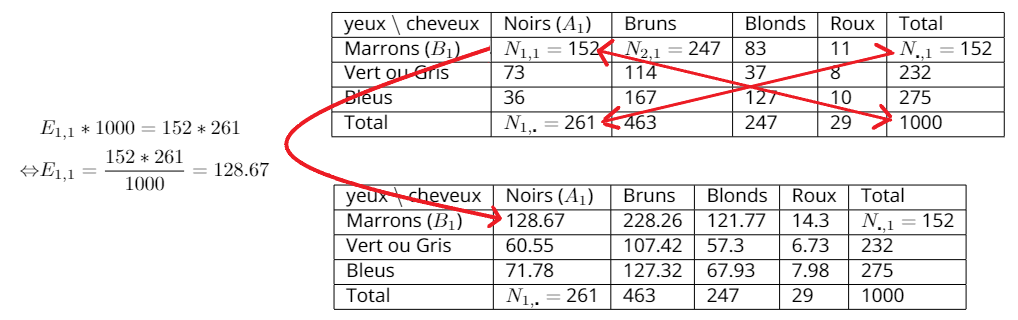
\includegraphics[width=.65\textwidth]{fig1_test.png}
\end{figure}
Puis calculer la stat de test 
\[
    D = \sum_{\text{chaque case du tableau}}\frac{N_{1,1}- E_{1,1}}{E_{1,1}}
.\]


\section{Test du $ \mathcal{X}^2 $ d'homogénéité}
\subsection*{Donnée}
\begin{itemize}
    \item $ X_1, \dots, X_{n_1} $ échantillons iid
    \item $ Y_1, \dots, Y_{n_2} $ échantillons iid
    \item Échantillons indépendant entre eux
\end{itemize}
Les variables sont toutes à valeurs dans les mêmes classes $ A_1, \dots, A_M $.

\subsection*{Conditions}
\subsection*{Hypothèse}
On veut tester l'homogénéité \begin{itemize}
    \item $ H_0 = X_1$ et $ Y_1 $  ont la même loi $ \Leftrightarrow \forall m \in \{1,\dots,M \}, P(X_1 \in A_m) = P(Y_1 \in A_m) $ 
    \item $ H_1 = X_1$ et $ Y_1 $  n'ont pas la même loi $ \Leftrightarrow \exists m \in \{1, \dots, M\} $ tel que $ P(X_1 \in A_m) \neq P(Y_1 \in A_m) $ 
\end{itemize}
\subsection*{Statistique de test}
\subsection*{Zone de Rejet}
\subsection*{Méthode}

\section{Test sur les Gaussiennes}
\subsection{Sur la moyenne}
\begin{itemize}
    \item Test sur 1 échantillon : Loi de Student \begin{itemize}
        \item Variance connu : on l'utilise à la place de $ V_n $ 
        \item Variance inconnu : On utilise $ \bar{X}_n $ dans $ V_n $ 
    \end{itemize}
    
    \item Test sur 2 échantillons indépendants : \begin{itemize}
        \item Variances connus :  
        \item Même variance inconnu : $ \bar{X}_{n_1} - \bar{Y}_{n_2} \sim \mathcal{N}(m_1 - m_2, \sigma ^2 (\frac{1}{n_1} + \frac{1}{n_2}))$ Same stat de test sauf qu'on estime la variance avec $ W = \frac{(n_1 - 1) V_{n_1}^X + (n_2 - 1) V_{n_2}^Y}{n_1 + n_2 - 2}$
        \item Variance inconnu : Test de welch : $ D = \frac{\bar{X}_{n_1} - \bar{Y}_{n_2}}{\sqrt[]{\frac{V_{n_1}^X}{n_1} + \frac{V_{n_2}^Y}{n_2}}} \sim_{H_0} \mathcal{T}(\mu ) $ avec $ \mu $ Formule horrible  
    \end{itemize}

    \item Test sur 2 échantillons apparié : $ Z_n $ into student (pas trouvé de raison yet)
\end{itemize}

\subsection{Sur la variance}
\begin{itemize}
    \item Test sur 1 échantillon : Comme le semestre d'avant \begin{itemize}
        \item Moyenne connu : On l'utilise dans le calcul de $ V_n $ 
        \item Moyenne inconnu : On utilise $ \bar{X}_n $ dans le calcul de $ V_n $ 
    \end{itemize}
    
    \item Test sur 2 échantillons indépendants : \begin{itemize}
        \item Moyennes connus : L'utiliser dans les calcul des $ V_n $ 
        \item Même Moyenne inconnu : X Pas de solution so do same as before
        \item Moyenne inconnu : $ D = \frac{X_{n_1}^X}{V_{n_2}^Y} $ qui suit $ \mathcal{F}(n_1 - 1, n_2 - 1) $ sans besoin de transformation.
    \end{itemize}

    \item Test sur 2 échantillons apparié : X
\end{itemize}

\section{Test de la somme des rangs aka MWW}
C'est le test de sur l'ordre stochastique.

\subsection*{Donnée}
\begin{itemize}
    \item $ X_1, \dots, X_{n_1}  $ iid. 
    \item $ Y_1, \dots, Y_{n_2}  $ iid.
    \item Échantillons indépendants
    \item On suppose que $ F_X $ et $ F_Y $ sont \textbf{continues}.
\end{itemize}

\subsection*{Conditions}
\begin{itemize}
    \item On suppose que $ F_X $ et $ F_Y $ sont \textbf{continues}.
    \item Mieux qu'un KS à deux échantillons !
\end{itemize}


\subsection*{Hypothèse}
\begin{itemize}
    \item $ H_0 = X_1 $ et $ Y_1 $ ont la même loi. $ F_{X_1} = F_{Y_1} $ 
    \item $ H_0 = X_1 $ et $ Y_1 $ n'ont pas la même loi. $ F_{X_1} neq F_{Y_1} $ \begin{itemize}
        \item Ou $ X_1 \succ Y_1 $ C'est à dire $ F_{X_1} \neq F_{Y_1} $ et $ \forall t \in \mathbb{R}, F_{Y_1}(t) \leq F_{X_1}(t) $ 
        \item Ou $ Y_1 \succ X_1 $ C'est à dire $ F_{X_1} \neq F_{Y_1} $ et $ \forall t \in \mathbb{R}, F_{X_1}(t) \leq F_{Y_1}(t) $ 
    \end{itemize}
\end{itemize}

\subsection*{Statistique de test}
\[
    U = \sum_{i=1}^{n_1}R(i) = \sum_{i=1}^{n_1} \sum_{j=1}^{n}\mathbbm{1}_{X_i \leq Z_j}
.\]
\begin{rem}[]
    En cas d'ex-æquo, on leur attribue le rang moyen des rangs. Voir exemple.
\end{rem}

\subsection*{Zone de Rejet}
La loi est symétrique. On a uniquement la table d'un côté, il faut calculer l'autre coté $ h_{1- \alpha} = h_\alpha + 2(\frac{n_1 n+1}{2} - h_\alpha )=  $.

Si $ n $ est grand, on utilise le TCL suivant 
\[
    \frac{U - E(U)}{\sqrt[]{Var(U)}} = \frac{U - n \frac{n_1 + 1}{2}}{\sqrt[]{\frac{n_1 n_2 (n+1)}{12}}} \to Z \sim \mathcal{N}(0,1)
.\]

\subsection*{Méthode}
On trie les données :
\begin{table}[!ht]
    \centering
    \begin{tabular}{|l|l|l|l|l|l|l|l|l|l|}
    \hline
        Obs & \textbf{5.6} & 7.4 & 9.6 & 11 & 12.6 & 12.6 & \textbf{12.8} & 13 &  \\ \hline
        Rang & 1 & 2 & 3 & 4 & 5.5 & 5.5 & 7 & 8 &  \\ \hline
        Obs & 14.8 & \textbf{15} & \textbf{15.2} & 15.4 & \textbf{15.6} & 15.6 & \textbf{16.4} & \textbf{16.4} & \textbf{18.8} \\ \hline
        Rang & 9 & 10 & 11 & 12 & 13.5 & 13.5 & 15.5 & 15.5 & 17 \\ \hline
    \end{tabular}
\end{table}
On calcule
\begin{align*}
    U &= 1 + 7 + 10 + 11 + 13.5 + 15.5 + 15.5 + 17 \\ 
        &= \text{Somme des rangs de } X_i = 90.5
\end{align*}

\section{Test du signe}
\subsection*{Donnée}
\begin{itemize}
    \item $ X_1, \dots, X_{n_1}  $ iid. 
    \item $ Y_1, \dots, Y_{n_2}  $ iid. 
    \item Échantillon \textbf{appariées} $ (X_1, Y_1), \dots, (X_n, Y_n) $ sont iid $ X_1 \not \bot Y_1 $ 
\end{itemize}
On note $ Z_i = Y_i - X_i $. On suppose que $ Z_i $  a une fonction de répartition continue donc aucun des $ Z_i $ ne vaut 0.

\subsection*{Conditions}
Fonction de répartition continue.

\subsection*{Hypothèse}
\begin{itemize}
    \item $ H_0 $ La médiane de $ Z $ vaut 0. $ m_Z = 0 $. C'est à dire que $ P(Y_1 < X_1) = 1/2 $ 
    \item $ H_1 = m_Z \neq 0 $ ou $ m_Z > 0 \Leftrightarrow P(Z \leq 0) > 1/2 \Leftrightarrow P(Y_1 > X_1) > 1/2$ ou $ m_Z < 0 $ 
\end{itemize}

\subsection*{Statistique de test}
\begin{align*}
    S_n &= \sum_{i=1}^{n}\mathbbm{1}_{Z_i \leq 0} \\
    &= \text{ Nombre de } Y_i > X_i
\end{align*}

\subsection*{Zone de Rejet}
\begin{itemize}
    \item Sous $ H_0 : P(Z_i > 0) = P(Y_i > X_i) = \frac{1}{2} $ 
    \[
        \mathbbm{1}_{Z_i > 0} \sim Ber(\frac{1}{2})
    .\]
    donc 
    \[
        S_n \sim Bin(n,\frac{1}{2})
    .\]

    \item Sous $ H_1 $ \begin{itemize}
        \item Si $ m_z > 0, P(Y_i > X_i) > \frac{1}{2}, S_n \sim Bin(n,p), p> \frac{1}{2} $ donc $ S_n $ est "grand"
        \item Si $ m_z < 0, P(Y_i < X_i) > \frac{1}{2} $ donc $ S_n $ est petit.
        \item Si $ m_z \neq  0, S_n $ a un comportement proche des extremes (petit/grand).
    \end{itemize}
\end{itemize}

On utilise donc une table de la loi binomiale. Si n est grand, on utilise le TCL.
\subsection*{Méthode}


\end{document}